\documentclass[professionalfonts,aspectratio=169]{beamer}

\usetheme{Madrid}
\usecolortheme{default}

% Changement ici : on passe le document en français pour la gestion des espaces et de la typographie
\usepackage[english]{babel} 
\usepackage{amsmath,amssymb}
\usepackage{graphicx}
\usepackage{booktabs}
\usepackage{hyperref}
\usepackage{listings}
\usepackage{color}

\lstset{language = Python,
        basicstyle = \ttfamily\small,
        keywordstyle = \color{blue},
        commentstyle = \color{gray},
        showstringspaces = false,
        breaklines = true}


%=============================================================================================


\setbeamersize{text margin left=5mm, text margin right=5mm}
\sloppy
\emergencystretch=3em

\title{Nouvelle structure pour les données opérationnelles dans la base de données LNCMI}
\author{Wolali KOFFI}
\institute{Master CSMI \\
           Université de Strasbourg \\[0.3 cm]
           En collaboration avec le CNRS et le LNCMI}
\date{Année universitaire 2025--2026}


%=============================================================================================


\begin{document}

\begin{frame}
    \titlepage
\end{frame}

\addtobeamertemplate{footline}{}{%
    \begin{beamercolorbox}[wd=\paperwidth,ht=2.5ex,dp=1.2ex,leftskip=1em]{author in head/foot}
        \usebeamerfont{author in head/foot}
        Master CSMI -- Université de Strasbourg
    \end{beamercolorbox}
}


%=============================================================================================


\begin{frame}{Contexte : Environnement de recherche}
    \begin{itemize}

        \item \textbf{CNRS} (Centre National de la Recherche Scientifique)
        \begin{itemize}
            \item Plus grand centre de recherche de France 
        \end{itemize}

        \item \textbf{LNCMI} (Laboratoire National des Champs Magnétiques Intenses)
        \begin{itemize}
            \item Organisation nationale qui fournit des champs magnétiques intenses pour la recherche scientifique
            \item Membre de l'\textbf{EMFL} (European Magnetic Field Laboratory)
            \begin{itemize}
                \item Fournit des accès à des champs magnétiques intenses pour la recherche scientifique internationale
            \end{itemize}
        \end{itemize}
        
    \end{itemize}
\end{frame}


%---------------------------------------------------------------------------------------------


\begin{frame}{Contexte : Origine du projet}
    \vspace{0.3cm}
    
    \begin{itemize}
        \item \textbf{Continuité académique}
        \begin{itemize}
            \item Suite directe des projets de développement réalisés en Master 1 CSMI.
            \item Focus sur l'algorithmie et le traitement de données scientifiques.
        \end{itemize}
        
        \vspace{0.4cm}
        
        \item \textbf{Travaux préliminaires (Projets M1)}
        \begin{itemize}
            \item Étude des problématiques liées aux séries temporelles massives.
            \item Développement d'algorithmes de sous-échantillonnage intelligent pour la visualisation (LTTB, M4, Min-Max).
        \end{itemize}
    \end{itemize}

\end{frame}



%---------------------------------------------------------------------------------------------


\begin{frame}{Objectifs du stage (2 mois)}
    
    \begin{itemize}
        \item \textbf{Intégration des travaux de projets (M1)}
        \begin{itemize}
            \item Déployer les algorithmes et pipelines développés précédemment.
        \end{itemize}
        
        \vspace{0.3cm}
        
        \item \textbf{Restructuration des enregistrements en base de données}
        \begin{itemize}
            \item \textbf{Architecture :} Intégration des vues TDMS (pupitre, archives, défauts), Site (Assembly), Housing (ex: M9), et paramètres d'alimentation.
            \item \textbf{Enrichissement des métadonnées :}
            \begin{itemize}
                \item Signatures du champ magnétique (pour le \textit{clustering}).
                \item Signatures des courants de référence (modèles de circuits ODE via \textit{magnet-scipy}).
                \item Statistiques globales (énergie) et suivi de la fatigue (cycles de contraintes).
            \end{itemize}
        \end{itemize}
        
        \vspace{0.3cm}
        
        \item \textbf{Développement de tableaux de bord (Dashboards)}
        \begin{itemize}
            \item Créer des interfaces visuelles interactives pour explorer et exploiter ces nouvelles structures de données.
        \end{itemize}
    \end{itemize}

\end{frame}

%=============================================================================================

\section{Réalisations}

\begin{frame}{Réalisations : Définition d'un « Site »}
    \begin{columns}[T] % L'option [T] aligne le texte vers le haut
        
        % Colonne de gauche pour l'image
        \begin{column}{0.45\textwidth}
            \centering
            % Assure-toi que l'image site.png est dans le même dossier que ton fichier .tex
            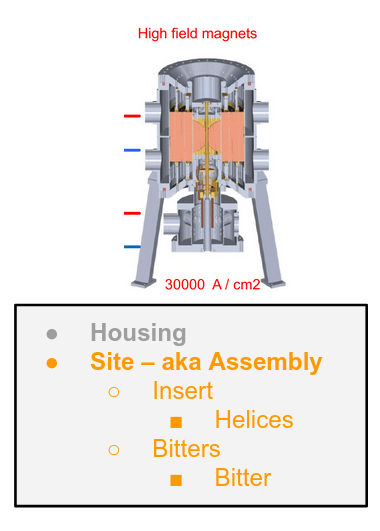
\includegraphics[height=0.75\textheight]{site.png}
        \end{column}
        
        % Colonne de droite pour les explications
        \begin{column}{0.55\textwidth}
            \textbf{Le Site (ou Assemblage)}
            \vspace{0.3cm}
            \begin{itemize}
                \item Représente le \textbf{cœur actif} de l'aimant à haut champ.
                \item S'insère dans une structure externe appelée \textit{Housing}.
                
                \vspace{0.4cm}
                
                \item \textbf{Composition interne de l'assemblage :}
                \begin{itemize}
                    \item \textbf{Insert} : Composé d'un système d'hélices.
                    \item \textbf{Bitters} : Empilement de disques de Bitter.
                \end{itemize}
            \end{itemize}
        \end{column}
        
    \end{columns}
\end{frame}

%---------------------------------------------------------------------------------------------

\begin{frame}{Réalisations : Pipeline et hiérarchie des données}
    \begin{center}
        \Large
        \textbf{Site} \quad $\xrightarrow{\text{utilisé pour}}$ \quad \textbf{Experiments} \quad $\xrightarrow{\text{génèrent}}$ \quad \textbf{Files}
    \end{center}
    
    \vspace{0.8cm}
    
    \begin{itemize}
        \item \textbf{1. Site (L'infrastructure matérielle)}
        \begin{itemize}
            \item La configuration physique exacte de l'aimant à un instant donné.
        \end{itemize}
        
        \vspace{0.4cm}
        
        \item \textbf{2. Experiments}
        \begin{itemize}
            \item Les différentes sessions de recherche ou tests de mise en service menés sur ce Site précis.
        \end{itemize}
        
        \vspace{0.4cm}
        
        \item \textbf{3. Files (Les données brutes opérationnelles)}
        \begin{itemize}
            \item Les enregistrements réels des capteurs rattachés à l'expérience.
        \end{itemize}
    \end{itemize}
\end{frame}


%=============================================================================================


\begin{frame}{Remerciements}
    \vspace{0.5cm}
    Je tiens à exprimer ma plus profonde gratitude à mes superviseurs et collaborateurs pour leurs conseils, leur expertise et leur soutien tout au long de ce projet :
    
    \vspace{0.6cm}
    
    \begin{itemize}
        \item[] \textbf{Christophe Trophime} (CNRS / LNCMI)
        \vspace{0.3cm}
        \item[] \textbf{Joubine Aghili} (IRMA)
    \end{itemize}
    
    \vspace{0.8cm}
    
    \begin{center}
        \small \textit{Un remerciement particulier à l'équipe pédagogique du Master CSMI de l'Université de Strasbourg.}
    \end{center}
\end{frame}


%---------------------------------------------------------------------------------------------


\begin{frame}
    \vspace{1.5cm}
    \begin{center}
        \Huge{\textbf{Merci de votre attention !}}
        
        \vspace{1.5cm}
        
        \Large{\textbf{Avez-vous des questions ?}}
    \end{center}
\end{frame}


%=============================================================================================
\end{document}